

\chapter{Theory of Single Vector Bosons}
The vector boson production cross section measurement during hadron collision, provides a deep understanding of quantum chromodynamics (QCD) and electroweak (EW) processes. The production of $W$ and $Z$ bosons are best examples of hard scattering processes at Large Hadron Collider. Theoretical predictions in perturbative chromodynamics are available at next-to-next-to-leading order~(NNLO)~\cite{PhysRevD.51.44, VANNEERVEN199211}.
 
The cross sections of $Z$ and $W$ boson and their ratios are experimentally measured by the ATLAS and CMS detector at the Large Hadron Collider~(LHC) in  proton-proton collisions at various center of mass energies. This thesis presents theoretically predicted cross section of the $W$ and $Z$ boson production cross section in a proton proton collision at $\sqrt{s}=13~TeV$~\cite{2016601}.

\section{Significance of $W$ and $Z$ Boson Production Cross Section}
The $W$ and $Z$ electroweak bosons were discovered at UA1~\cite{UA1:1983crd} and UA2~\cite{UA2:1983mlz}, and their detailed measurements have been done at electron-positron and hadron Collider. LEP~(Linear electron-positron) performed many accurate measurements for the study of these vector bosons, with a precision of $1~\%$~\cite{guageboson}. At Large hadron colliders, single vector boson production has been performed  at various center of mass~(C.O.M) energies i.e. $\sqrt{0.63}~TeV$ at the CERN S$p\overline{p}$S~(Super Proton Anti proton Synchrotron) by UA1 and UA2, at $\sqrt{1.8}~TeV$ at the Tevatron by CDF~(Collider Detector at Fermi lab)~\cite{PhysRevLett.62.1005} and  at $\sqrt{1.96}~TeV$ by D0~(DZero)~\cite{PhysRevLett.100.102002}. There are large number of $W$ and $Z$ events produced in Large Hadron Collider, which help us to measure production cross section of these bosons easily, roughly around 140,000 events for $Z\rightarrow ee$ and 500,000 $W\rightarrow e\nu$ events are recorded with $2.2~fb^{-1}$ of data. Measurements of production cross section of vector bosons at the $Sp\overline{p}S$ and the Tevatron are very important, as these measurements provide data for the development of leading-order~(LO) and next-to-leading order~(NLO) theoretical predictions and results of these measurements are also used for comparison with data at the LHC. LHC provides measurement of $W$ and $Z$ boson at higher energy regimes, so we can improve our  theory of perturbative Quantum Chromodynamics~(QCD). The results at higher energy regime also provide more constraints on the parton distribution function~(PDF) along with improvement in electroweak precision measurements, i.e mass of charged vector boson $W$ and $sin^{2}\theta$. These new measurements of vector bosons at LHC provide deep insight for the study of new physics including measurement of Higgs boson parameters, top quark physics and physics beyond the standard model.\\
Increase in energy at LHC benefits for the predictions of perturbative QCD, Fig.~\ref{fig1} illustrates these benefits.  We can reach further lower Bjorken $x-$value for any process, e.g the production of $Z$ vector boson shown here. With these new energy regimes we can reach more low $x$ region as compared to SPS and Tevatron experiments. This may improve statistical and systematic uncertainties. Millions of vector boson events have been detected at CMS and ATLAS experiments. These new detectors can measure electrons up to to $|\eta|<4.9$ and jets to $|\eta|<4.4$ and a large fraction of low-$x$ events can be reconstructed by the LHC detectors.   


\section{Theory of Single Vector Boson Production}
The theoretical predictions used for comparison of $W$ and $Z$ boson production cross section have been improved. The theoretical predictions in perturbative QCD theory are available up to next-to-next-to-leading order~(NNLO). Theoretical predictions at next-to-leading order(NLO) for the production cross section of vector boson in association with jets exist for five partons in the final state. The uncertainties in  theoretical prediction  are comparable with experimental uncertainties. We will discuss about different types of theoretical uncertainties in last section of this chapter.
\begin{figure}{h!}
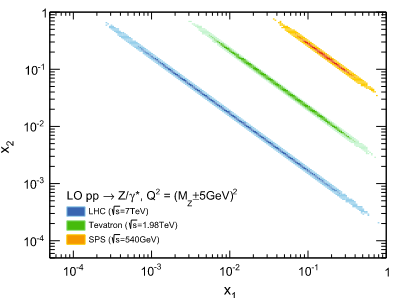
\includegraphics[scale=1]{chapter3/bjorkenx.png}
\caption{Correlation of LHC, Tevatron and SPS hadron Collider between the $x$ values of the interaction of two partons~\cite{Schott_2014}}.
\label{fig1}
\end{figure}
 
\subsection{Cross Section Calculation}
There are two energy regimes for the calculation of production cross section in proton-proton collisions at Large Hadron Collision(LHC)
\begin{itemize}
\item High-energy regime also called short distance regime
\item Low-energy regime also called long distance regime
\end{itemize}
In perturbative QCD there are two terms in the factorization theorem: one is $\hat{\sigma}_{q\overline{q}}\rightarrow n$ at short-distances for the parton-parton interaction and other is for large distances and explain the internal structure of proton. In case of very large momentum transfer $q$ in the interaction of parton, the interactions can be evaluated with perturbative QCD theory. The long-distance term or for low momentum transfer $q$, where perturbative QCD theory can not be applied, parton density function~(PDFs) describes the proton structure. These PDFs Functions can be written as $f_{\frac{a}{A}}(x,Q^{2})$ for the parton $a$ in the proton $A$, in which $x=\frac{p_{a}}{p_{A}}$ is shared momentum fraction for parton $a$ from proton's momentum and $Q^{2}$ is the energy scale of the scattering process.\\
The long-distance physics or physics at low momentum transfer and short distance physics or physics at high momentum transfer in parton-parton interaction, is separated by a scale called factorization scale $\mu_{F}=Q$~\cite{Mukhi:2019yrf}.
The cross section in the interaction of proton-proton is expressed by  
\begin{equation}
\sigma_{p_{A}p_{B}\rightarrow n}=\Sigma_{q}\int dx_{a}dx_{b}f_{\frac{a}{A}}(x_{a},Q^{2})\times f_{\frac{b}{B}}(x_{b},Q^{2})\hat{\sigma}_{ab\rightarrow n}
\end{equation}   
\begin{figure}[h!]
\centering
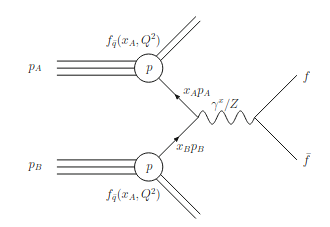
\includegraphics[scale=0.7]{chapter3/pdf.png}
\caption{Schematic of proton-proton collision at LHC.}
\label{p-p-collision}
\end{figure}
as shown in Figure~\ref{p-p-collision}. $f_{\frac{a}{A}}$ denotes the PDF of parton $a$ and $f_{\frac{b}{B}}$ is for parton $b$ in protons $A$ and $B$ respectively. All quark flavours are included in the sum and integration is performed over momentum fraction of parton $a$, $x_{a}$ and momentum fraction of parton $b$, $x_{b}$.\\
If we include the QCD corrections, then parton-parton cross section in term of $\alpha_{s}$ is,
\begin{equation}\label{qcd-correct}
\sigma_{p_{A}p_{B}\rightarrow n}=\Sigma_{q}\int dx_{a}dx_{b}f_{\frac{a}{A}}(x_{a},Q^{2})f_{\frac{b}{B}}(x_{b},Q^{2})\times[\hat{\sigma}_{0}+\alpha_{s}(\mu_{R}^{2})\hat{\sigma}_{1}+....]_{ab\rightarrow n}
\end{equation}
In Equation~\ref{qcd-correct},~ $\sigma_{1}$ is the correction in parton-parton cross section of order one, and $\sigma_{0}$ is the base-level parton-parton cross section. Therefore reference scale for the running strong coupling constant $\alpha_{s}(\mu_{R}^{2})$ is set by $\mu_{R}$~(re-normalisation scale). The re-normalisation scale~\cite{Mukhi:2019yrf} is set to eliminate the ultraviolet divergences in finite order cross section calculations.

\subsection{Parton Distribution Functions}

The quantum numbers of a hadron are determined by valance quarks. For example proton has two up quarks~($u_{v}$) and one down quark~($d_{v}$) and neutron has one up quark~($u_{v}$) and two down quarks~($d_{v}$). Along with these valance quarks, there are many quarks and anti quarks inside hadrons due to presence of gluons.
Deep Inelastic Scattering~(DIS)~experiments are best to probe the internal structure of nucleons, in which lepton acts as a probe by transferring four momentum $|q|$ to the nucleon in the collision. Electron-proton DIS experiment at SLAC in 1966 was the first evidence for the parton structure inside nucleons.\\
The resolving power of probe in DIS is~$\approx~\frac{\hbar}{|q|}$, and the level of structure that can be revealed is increased with $|q|$~i.e. we can get a resolution of $0.002~fm$ at $|q|=~100~GeV$, which is enough to probe the internal structure of proton.\\
The momentum distribution function of parton within nucleons is simply called Parton Distribution Function~(PDF). The PDF gives the probability~(normalised to the number of partons)~of finding the parton with momentum fraction $x$ at an energy scale $Q^{2}=-q^{2}$. DIS experiments show that at low $Q^{2}$ the three valance quarks are more and more dominant. For the high $Q^{2}$ values there will be many quark-antiquark pairs with low momentum fraction $x$. The result of DIS experiments show that, $\approx50\%$ of nucleon's momentum is carried by quarks and antiquarks and remaining is carried by gluons, momentum fraction carried by gluons is increased with $Q^{2}$. 
QCD predicts how parton distribution changes with $Q^{2}$ energy scale and these predictions are governed by the QCD evolution equation DGLAP in perturbative QCD domain, that is where the value of $\alpha_{s}(Q^{2})$ is much smaller than one. There are different levels of approximations for DGLAP equation, relative to the power of $\alpha_{s}(Q^{2})$ in the perturbative domain, named as Leading-Order~(LO),~i.e. first order in $\alpha_{s}(Q^{2})$, Next-to-Leading-Order~(NLO) and Next-to-Next-to-Leading-Order~(NNLO). The Parton Distribution Function~(PDF) has an essential role in calculation of cross section. A PDF  $f_{i}(x,~\mu_{F},~\mu_{R})$ gives the probability of finding a parton $i$ with a momentum fraction $x$ with factorisation and re-normalisation scale $\mu_{F}$, and $\mu_{R}$, where $\mu_{F}$ is also called the probed scale of scattering experiment. The factorisation and re-normalisation~\cite{Mukhi:2019yrf} scale parameters $\mu_{F}$ and $\mu_{R}$ are used to prohibit infrared and ultraviolet divergences. For the hard scattering processes these scales are of the order of momentum scale~i.e. for the Drell-Yan process~\cite{Peng:2016ebs} these scales have typical value which implies $\mu_{F}=\mu_{R}=m_{Z}$. Usually both scales are equal. For the prediction of cross sections these scale are varied simultaneously within $0.5Q<\mu_{F},\mu_{R}<2.0Q$, where $Q$ is the probe scale of the scattering process.\\
Perturbative QCD theory cannot predict the actual mathematical form of PDF $f_{i}(x,~\mu_{F})$, it gives $Q^{2}$ dependence but cannot predict dependence of parton distributions function on $x$ at given $Q^{2}$. Data from Deep inelastic scattering experiments~(DIS), are the main source of PDF determination. \\
For PDFs fit to data, a starting scale is chosen where perturbative QCD predictions can be applied, and we assume many functional forms of the PDFs.  Parametrisation of the PDF $f_{i}(x,\mu_{F})$ takes the form 
\begin{equation}
f-{i}(x,~\mu_{F})=a_{0}x^{a1}(1-x)^{a_{2}}P(x,~a_{3},~a_{4},~...)
\end{equation}   
In which $P$ is a polynomial function and $a_{j}$ is experimentally measured fit value that can not be theoretically predicted. In second step, we choose factorisation scheme, this scheme modeled how heavy quarks are treated, and an order of perturbation theory to be used. 
\begin{figure}[h!]
\centering
\begin{tabular}{c}
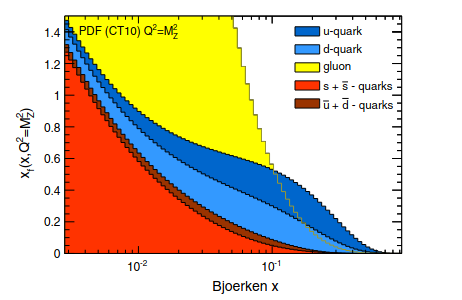
\includegraphics[scale=0.8]{chapter3/cteq-pdf.png}\\

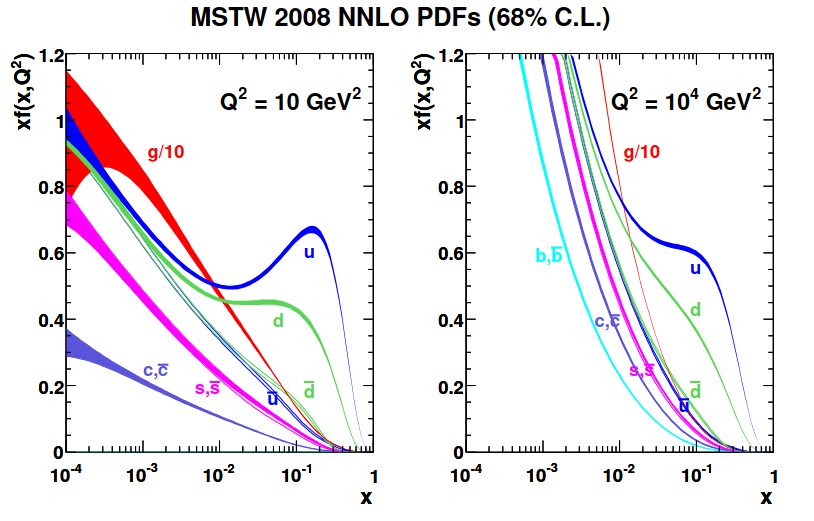
\includegraphics[scale=0.5]{chapter3/pdf1.png}
\end{tabular}
\caption{Parton Distribution Function evaluated at $Q^{2}=m_{Z}^{2}$~\textit{top}~\cite{Schott_2014}, MSTW 2008 NNLO PDFs at $Q^{2} = 10 GeV^{2} $and $Q^{2} = 10^{4} GeV^{2}$~\textit{bottom}~\cite{Martin_2009}}
\label{pdf-fit}
\end{figure}

There are several groups who performed PDFs fitting. The results of CTEQ~\cite{Nadolsky_2008}, MSTW~\cite{Martin_2009}, ABKM~\cite{Alekhin_2010} and NNPDF~\cite{Ball:2011us} collaborations some of which are shown in Fig.~\ref{pdf-fit}, use all available data for their fits. There are several assumptions and model uncertainties on which PDF approach and fitting is based.\\
There are different multi purpose event generators, which include all the theoretical aspects of the proton-proton collision. These events generators use different theoretical models which include, shower model for initial and final MPI model~\cite{Blok_2016} and hadronisation and final decay model. Some frequently used generators are PYTHIA~\cite{Sj_strand_2008}, HERWIG~\cite{Corcella_2001}, SHERPA~\cite{Gleisberg_2009} and POWHEG~\cite{Oleari_2010}. These generators have all aspects of Standard Model and new physics. The detail of each generator, and what it can do can be found in~\cite{Schott_2014}. 

\section{Measurement of Cross Section at The LHC}
Experimentally, the production cross section is measured by the following equation:
\begin{equation}
\sigma_{V}^{inc}=\frac{N_{signal}}{\epsilon.BR.\int \mathcal{L}dt}
\end{equation}
where $N_{signal}=N_{data}-N_{bkg}$ which is number of signal events, $N_{data}$ is the number of selected events from data and $N_{bkg}$ are the background events. The factor $\epsilon$ depends on determination of criteria for the signal selection. To specify the decay channel of $W$ and $Z$ boson branching ratio factor~(BR) is used. Integrated luminosity $\int \mathcal{L}dt$, tells about the size of data sample used.\\
The $\epsilon$ is defined as :
\begin{equation}
\epsilon=\frac{N_{reco.}^{selected}}{N_{gen.}^{all}}
\end{equation}
\begin{equation}
\epsilon=\frac{N_{reco.}^{selected}}{N_{gen.}^{selected}}.\frac{N_{gen.}^{selected}}{N_{gen.}^{all}}
\end{equation}
\begin{equation}
\epsilon=C.A
\end{equation}
where $N_{reco.}^{selected}$ are events selected at the reconstruction level and $N_{gen.}^{all}$ is the number of all generated events. $A$ represents fiducial acceptance factor and $C$ is for detector-induced correction factor. Ratio of the number of selected events at generator level~($N_{gen.}^{selected})$ to the total number of generated events~($N_{gen.}^{all}$)~ is called fiducial acceptance. The main source of uncertainties in the fiducial acceptance are scale and PDF uncertainties.\\
The detector correction factor $C$ is ratio of~($N_{reco.}^{selected}$) from data sample to the number of selected events~($N_{gen.}^{selected}$) from Monte Carlo. The dominant uncertainties in the detector correction factor are experimental sources.
The fiducial cross-section, defined as:
\begin{equation}
\sigma_{V}^{fid}=\frac{N_{data}-N_{bkg}}{C.BR.\int \mathcal{L}dt}=\sigma_{V}^{inc}.A
\end{equation}  
\section{Event Selection for Vector Bosons}
\subsubsection{ATLAS}
Events for $Z$ boson, i.e., $Z~\rightarrow~l^{+}l^{-}$ required Di lepton invariant mass of $66~GeV<~m_{ll}<116~GeV$. Muons must be in $|\eta|<2.4$ with $p_{T}(min.)~>~20~GeV$. Electrons are required to fulfill $1.52~<~|\eta|~<~2.4$ with $E_{T}(min.)>20GeV$.\\
$W$ boson decays to an energetic lepton and corresponding neutrino, neutrinos cannot be detected hence leads to missing transverse energy. Thus the mass of $W$ boson cannot be reconstructed due to this missing energy. The invariant mass projection to the transverse plane, defined as
\begin{equation}
m_{T}=\sqrt{2.p_{T}^{l}.p_{T}^{\nu}.(1-cos(\phi^{l}-\phi^{\nu}))}
\end{equation} 
can be reconstructed, where $p_{T}^{l}$ is lepton transverse momentum and $p_{T}^{\nu}$ is neutrino transverse momentum, $\phi^{l}$ and $\phi^{\nu}$ are azimuthal angles for lepton and neutrino respectively. For the $W$ boson events selection at ATLAS required one reconstructed, single lepton with $E_{T}^{miss.}$ of $25~GeV$ and $m_{T}(min.)~>~50~GeV$. Selection for the $Z$ boson by ATLAS is shown in Fig.~\ref{ATLAS_sel}
\begin{figure}[H]
\begin{tabular}{cc}

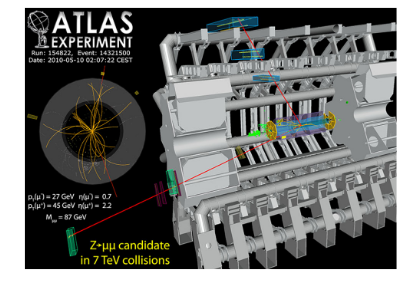
\includegraphics[scale=0.5]{chapter3/atlas.png}
&
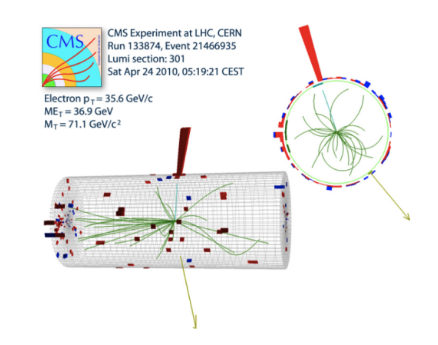
\includegraphics[scale=0.5]{chapter3/cms-w.png}
\end{tabular}
\caption{$Z\rightarrow \mu\mu$ in ATLAS detector~(left)~and $W\rightarrow e\nu$ in CMS detector~(right)~\cite{Schott_2014}.}
\label{ATLAS_sel}
\label{W-event}
\end{figure}
 
\subsubsection{CMS}
For $Z\rightarrow \mu\mu$, oppositely charged muons are required for $|\eta|<2.1$ and transverse momentum requirement of $p_{T}>20GeV$. For the electron decay channel $Z\rightarrow ee$, $|\eta|<1.44$ and $E_{T}>20$ GeV are required.\\
The selection criterion for $W$ boson events, required single electron with $E_{T}>25~GeV$ and $|\eta|<2.5$ or single muon with $p_{T}>25~GeV$ and $|\eta|<2.1$. A typical $W\rightarrow e\nu$ event in the CMS detector is shown in Fig.~\ref{W-event}. Tables \ref{Atlas_tab} and \ref{Cms_tab} show the kinematic cuts used by CMS and ATLAS.

\begin{table}[h!]
\centering
\caption{Kinematic cuts for CMS analysis~\cite{2011} at $7~TeV$ for leptonic channel of $Z$ and $W$ boson respectively.}
\begin{tabular}{|lp{5cm}p{5cm}|}
\hline
CMS&&\\
Electron-channel&$Z\rightarrow l^{+}l^{-}$ & $W\rightarrow l^{\pm}\nu$\\
\hline
&$E_{T}(e^{+})>25GeV$&one $ e^{\pm}$ with $E_{T}>25GeV$\\
&$E_{T}(e^{-})>25GeV$&$|\eta_{e^{\pm}}|<1.44$\\
&$|\eta_{e^{\pm}}|<1.44$&\\
&$60~GeV<m_{ee}<120~GeV$&\\
Muon-channel&&\\
\hline
&$p_{T}(\mu^{+})>25GeV$&one $ e^{\pm}$ with $p_{T}>25GeV$\\
&$p_{T}(\mu^{-})>25GeV$&$|\eta_{\mu^{\pm}}|<2.1$\\
&$|\eta_{\mu^{\pm}}|<2.1$&\\
&$60~GeV<m_{\mu\mu}<120~GeV$&\\
\hline
\end{tabular}
\label{Atlas_tab}
\end{table}

\begin{table}[h!]
\centering
\caption{Kinematic cuts for ATLAS analysis~\cite{Aad_2016} at $13~TeV$ for the leptonic channel of $Z$ and $W$ boson respectively.}
\begin{tabular}{|lp{5cm}p{5cm}|}
\hline
ATLAS&&\\
Electron-channel&$Z\rightarrow l^{+}l^{-}$ & $W\rightarrow l^{\pm}\nu$\\
\hline
&$E_{T}(e^{+})>25GeV$&$p_{T}^{(e^{\pm})}>25GeV$\\
&$E_{T}(e^{-})>25GeV$&$p_{T}^{(\nu)}>25Gev$\\
&$|\eta_{e^{\pm}}|<1.37$&$|\eta_{e^{\pm}}|<1.52$\\
&$66~GeV<m_{ee}<116~GeV$&$m_{T}>50GeV$\\
Muon-channel&&\\
\hline
&$p_{T}(\mu^{+})>25GeV$&$p_{T}^{(\mu^{\pm})}>25GeV$\\
&$p_{T}(\mu^{-})>25GeV$&$p_{T}^{(\nu)}>25GeV$\\
&$|\eta_{\mu^{\pm}}|<2.4$&$|\eta_{\mu^{\pm}}|<2.4$\\
&$66~GeV<m_{\mu\mu}<116~GeV$&$m_{T}>50GeV$\\
\hline
\end{tabular}
\label{Cms_tab}
\end{table}

\begin{figure}[h!]
\centering
\begin{tabular}{c}
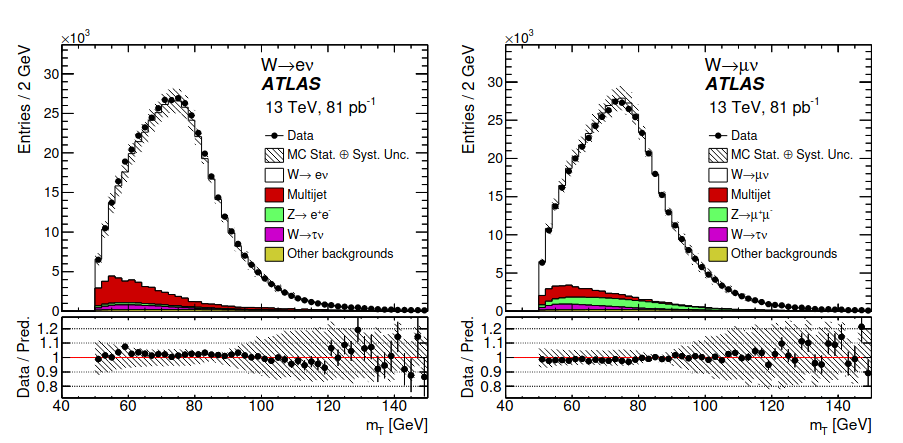
\includegraphics[scale=0.45]{chapter3/mt.png}\\

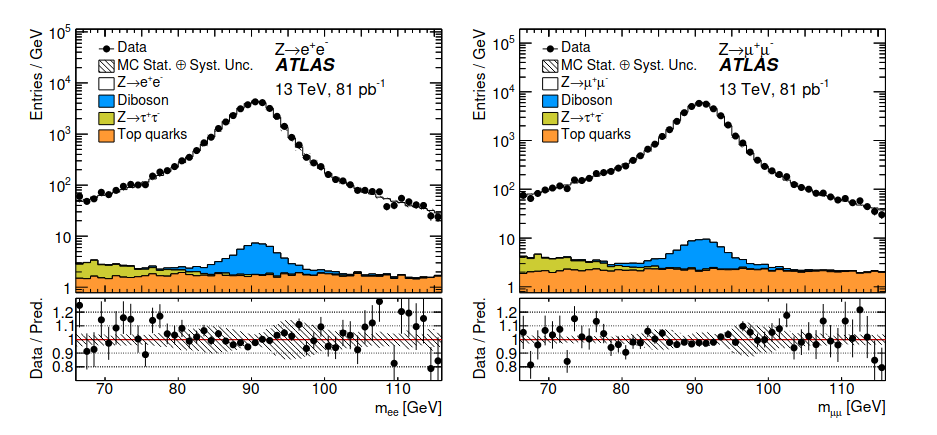
\includegraphics[scale=0.45]{chapter3/mll.png}
\end{tabular}
\caption{Transverse mass~$m_{t}$ distributions of $W\rightarrow e\nu$ and $W\rightarrow \mu\nu$ process~(top) and dilepton mass~$m_{ll}$ distribution~ (bottom)~\cite{Aad_2016}}
\label{mt_mll}
\end{figure}

The transverse mass distribution for electron and lepton channel of $W$ boson event and dilepton mass distribution for the $Z$ boson event can be seen in Fig.~\ref{mt_mll}. 
\section{Inclusive Cross Section of $W$ and $Z$ Bosons  }
For the Drell–Yan processes~\cite{Peng:2016ebs} as shown in Fig.~\ref{drell-yan}, the theoretical prediction at NNLO are known in term of $\alpha_{s}$~(strong coupling constant) for the inclusive production cross section of  the $Z$ and $W$ vector boson.\\
$Z$ bosons are produced by the quarks-antiquark annihilation, i.e. $u\overline{u}$, $d\overline{d}$ and also $s\overline{s}$. $W^{\pm}$ boson production is different from $Z$ boson because it depends on the charge of $W$, $W^{+}$ boson is produced in $u\overline{d}\rightarrow W^{+}$ process and $W^{-}$ in $d\overline{u}\rightarrow W^{-}$ process. $W^{+}$ is produced from the annihilation of $u-$valance quarks and $\overline{d}-$sea quark, $W^{-}$ from $d-$valance quark and $\overline{u}$ quark. Since there are two $u-$ quarks~(valance) and one $d-$ quark~(valance) available in the proton, therefore more $W^{+}$ bosons are expected than $W^{-}$ bosons. Thus QCD predictions can be tested precisely from the ratio of  $W^{+}$ and $W^{-}$ production as cross section ratios cancel many of the theoretical and experimental uncertainties.\\
\begin{figure}[H]
\begin{tabular}{c}
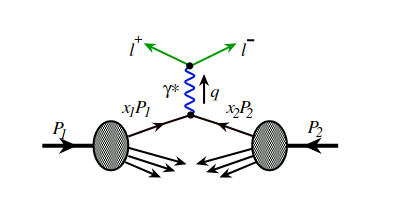
\includegraphics[scale=0.5]{chapter3/drell-yan1.png}
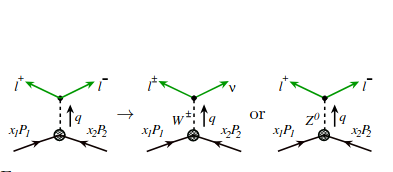
\includegraphics[scale=0.5]{chapter3/drell-yan2.png}
\end{tabular}
\caption{Graphical sketch for the generalized partonic
hard part of the Drell-Yan process~\cite{Peng:2016ebs}}
\label{drell-yan}
\end{figure}
Integrated luminosity is one of the main source of experimental uncertainties. In cross-section ratio measurement, this uncertainty is reduced, along with some other experimental and theoretical uncertainties.~Therefore along with cross-section of $W$ and $Z$ boson, cross section ratios $\frac{\sigma(W^{+}+\sigma(W^{-})}{\sigma(Z)}$ and $\frac{\sigma(W^{+})}{\sigma(W^{-})}$, have unique importance.\\
The cross-section ratio for $\sigma(W^{+}+W^{-})/\sigma(Z)$ represents the cross section dependence on the quarks-distribution functions.
 
 \begin{eqnarray}
\sigma(W^{+}+\sigma(W^{-})=u_{v}(x)+\overline{d}_{v}(x)+d_{v}(x)+\overline{u}_{s}(x)\\
\sigma(Z)=(g_{V}(u)^{2}+g_{A}(u)^{2}.u_{q}(x))+(g_{V}(d)^{2}+g_{A}(d)^{2}.v_{q}(x))
\end{eqnarray} 
with\\

\begin{equation}
u_{q}(x)=(u_{v}(x)+\overline{u}_{s}(x))
\end{equation}
\begin{equation}
v_{q}(x)=(d_{v}(x)+\overline{d}_{s}(x))  
\end{equation}
where $u_{v}(x)$ and $\overline{u}_{s}(x)$ are valance quark distributions and $u_{s}(x)$ and $d_{s}(x)$ are the respective sea-quark distributions.
If we assume that light sea quark and anti-quark have same distribution, then the PDF dependence will be reduced,~i.e, $\overline{q}(x) = q(x)$  for $q= u,d,s..$. Thus the ratio of $W$ to $Z$ boson helps us to constrain the strange quark distribution~\cite{Aad_2012}.\\
The above statement doesn't hold for cross-section ratios, such as ratio of $W^{+}$ to $W^{-}$, $W^{+}$ or $W^{-}$ to $Z$ boson. These cross section ratios have a large dependence on difference in the $u-$ and $d-$quark distribution functions, and is very sensitive to this difference in valance-quark distributions. However, for the PDFs constraints, along with inclusive cross section the differential cross section measurements are also very important. 

\subsection{Differential Production Cross Section of $W$ and $Z$ Boson:}
The differential cross section also measured at LHC with great precision, and differential cross section of vector bosons plotted versus their rapidity distribution, provides extra constraint on the PDFs.

Rapidity distribution for the process $Z\rightarrow l^{+}l^{-}$, can be directly measured from  detector data, because  four-momenta of the decaying leptons can be precisely measured and thus rapidity can be measured precisely. This will help us to constrain the PDFs of $u\overline{u}$, $d\overline{d}$, and $s\overline{s}$. The differential cross section measurement helps us to improve strange-quark PDFs. Fig.~\ref{raptdity-atlas} shows different quark/antiquark annihilation processes for different rapidity ($y_{Z}$) values.  The rapidity distribution of $Z$ boson from the annihilation of $u\overline{u}$, $d\overline{d}$ and $s\overline{s}$ processes gives additional constraints on PDFs, as well as the rapidity distribution in the central region for $s\overline{s}$ process, is important to determine its PDFs. 
ATLAS and CMS both, published differential cross section $\frac{d\sigma}{d|y_{z}|}$ for different integrated luminosities $\int\mathcal{L}dt$ in the fiducial region defined by kinematic cuts earlier.\\
The $W$ boson decays into lepton and corresponding neutrino,~i.e.,~$W^{\pm}\rightarrow l^{\pm}\nu$. The direct measurement of rapidity distribution of $W^{\pm}$ boson is not possible, because the $p_{z}$ of decayed neutrino can't be reconstructed, thus pseudo rapidity of the decay lepton $\eta_{l}$ is measured and correlated to $y_{W}$ by an indirect method.
The rapidity distribution of $W^{\pm}$ boson is sensitive to the $u\overline{d}$ and $d\overline{u}$~quark distribution as shown in Fig.~\ref{raptdity-atlas}. The $y_{Z}$ measurement helps us to constrain the PDFs of strange quark.\\
Differential cross-section measurements of the $W$ and $Z$ bosons provide important constraints for the PDFs. Fig.~\ref{ubsr-sbsr} shows the difference in  PDFs of $\overline{u}$ and $\overline{s}$ quarks with and without LHC data based on the NNPDF group.
\begin{figure}[H]
\centering
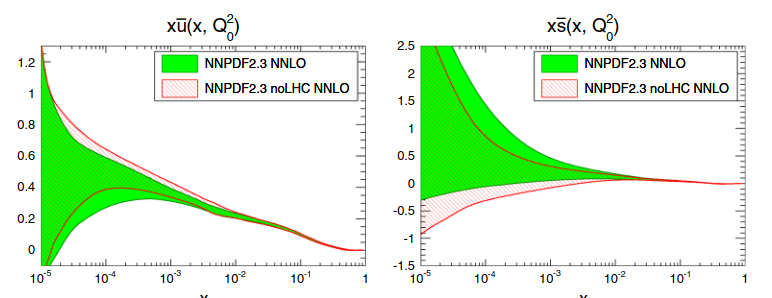
\includegraphics[scale=0.5]{chapter3/strange-quark.png}
\caption{Comparison of PDfs of $\overline{u}$ and $\overline{s}$~quark with LHC and without LHC data.~\cite{Schott_2014}. Comparison plots can also be found in~\cite{Ball_2013}.}
\label{ubsr-sbsr}
\end{figure}

\begin{figure}[H]
\centering
\begin{tabular}{c}
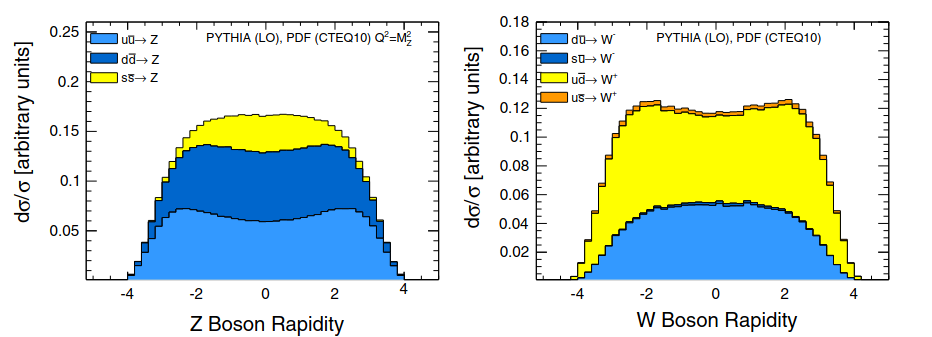
\includegraphics[scale=0.44]{chapter3/rapidity.png} \\
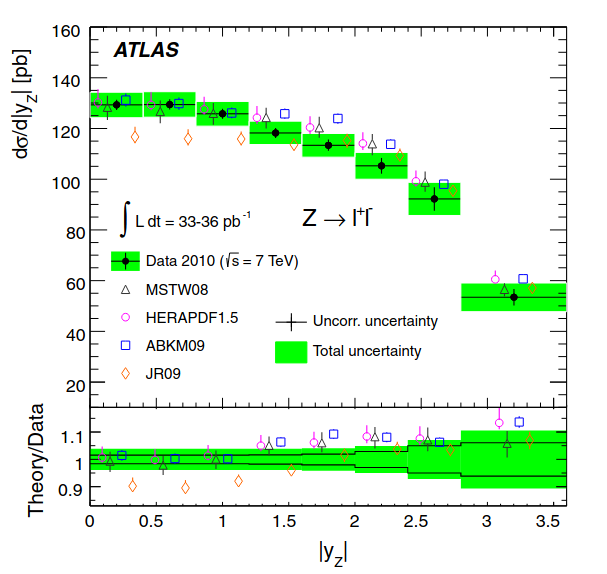
\includegraphics[scale=0.44]{chapter3/atlas-rapidity.png}
\end{tabular}
\caption{$Z$ boson rapidity distribution~(\textit{left}) and $W$ boson rapidity distribution~(\textit{right}) in 7 TeV pp collisions(\textit{top}), for $Z\rightarrow l^{+}l^{-}$ the combined $d\sigma/d|y_{Z}|$ cross-section measurement compared to NNLO theoretical predictions (\textit{bottom})~ \cite{Schott_2014}}.
\label{raptdity-atlas}
\end{figure} 


\section{Measurement of $p_{T}$ of Vector Bosons}
The $W$ boson mass at LHC can be measured by the accurate measurement and understanding of transverse momentum $p_{T}$, the $p_{T}$ distribution of product leptons of $W^{\pm}~\rightarrow~l^{\pm}\nu$ is an important parameter for $m_{W}$.\\
The $p_{T}$ distribution of electron and muon channel for the $Z\rightarrow l^{+}l^{-}$ process can be computed directly from four momentum information of resulting leptons.\\
The $p_{T}(Z)$ distribution is a important tool for the Monte-Carlo~(MC) generators, and transverse momentum of $Z$ boson helps to measure the $p_{T}(W)$, of which direct measurement is not possible.
The transverse momentum of  $W$ boson cannot be measured directly from the decayed leptons because we don't know about neutrino momentum. However, the $p_{T}~(W)$ is measured by the $p_{T}~(hadron)$ from which it was produced. The $p_{T}~(W)$ is balanced by the hadronic transverse momentum $p_{T}~(hadron)$, i.e.
\begin{equation}
p_{T}(W)=-p_{T}(had)=p_{T}(l^{\pm}+p_{T}(\nu)),
\end{equation}
where $p_{T}(had)$ is the recoil of hadron~(Fig. \ref{pt-w}),
\begin{figure}[h!]
\centering
\begin{tabular}{c}
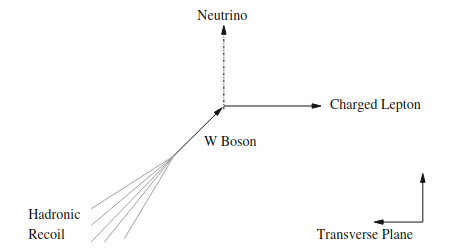
\includegraphics[scale=0.8]{chapter3/pt.png}\\
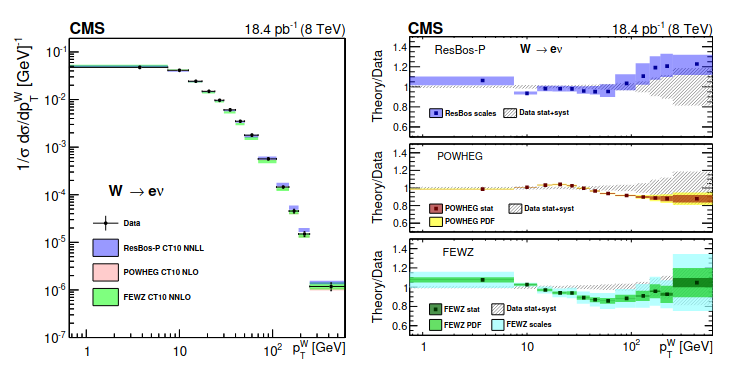
\includegraphics[scale=0.5]{chapter3/ptw.png}
\end{tabular}
\caption{Hadronic recoil illustration in $W^{\pm}~\rightarrow~ l^{\pm}\nu$ events~(\textit{top}). Differential cross sections~(Normalized) for $W$ boson as a function of $p_{T}~(W)$ for electron. Ratios of theoretical predictions to the data~(\textit{bottom}) ~\cite{Khachatryan_2017}.}
\label{pt-w}
\end{figure}
hence $p_{t}(W)$ can be measured from hadronic transverse momentum $p_{t}(hadron)$, which is due to hadronic activities in QCD interactions of hadrons. Due to several experimental uncertainties in the hadronic recoil, a theoretical model is used to define the relation between $p_{T}(had)$ and $p_{T}(W)$. Data of $Z$ boson events helps to model this theoretical model. We consider that the hadronic recoil $p_{T}~(hadron)$ is same for the $W$ and $Z$ bosons, and with different approach we can find $p_{T}~(W)$.

\section{Measured Cross Section of $W$ and $Z$ Bosons at Different C.O.M Energy}
The production cross section of $W$ and $Z$ vector bosons is measured at LHC in ATLAS and CMS experiments at different center-of-mass energies,~i.e., $7~TeV$, $8~TeV$ and $13~TeV$  with certain uncertainties~($\pm stat.\pm syst.\pm lumi.$). The measured value of cross section increased with the increase in center-of-mass energy as shown in Fig.~\ref{pred-inc}.
\begin{figure}[h!]
\centering
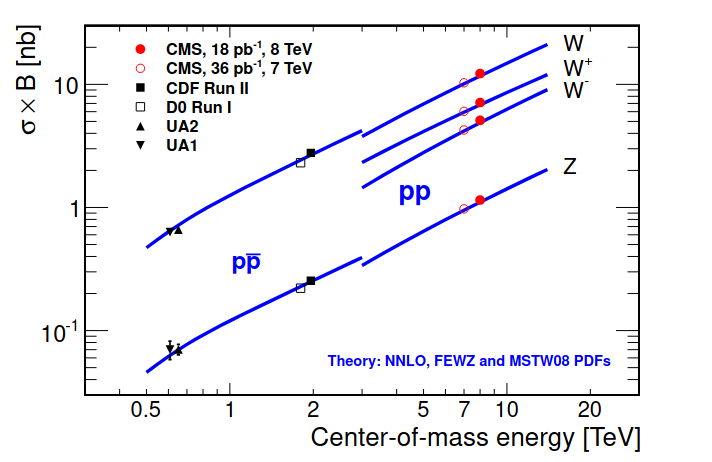
\includegraphics[scale=0.5]{chapter3/cross-sction-inc.png}
\caption{The predicted increase in cross section of vector bosons~\cite{Chatrchyan_2014}.}
\label{pred-inc}
\end{figure}
The production cross-section of $W$ and $Z$ boson, measured~$(\sigma\times BR(W\rightarrow l\nu, Z\rightarrow ll))$ and predicted at various c.o.m energies is listed in the following Tables \ref{7_1},~\ref{7_2},~\ref{8_1},~\ref{8_2},~\ref{13_1} and \ref{13_2}.


\begin{table}[H]
\caption{Measured and NNLO predicted Ratios of $W^{+}/W^{-}$ and $W^{\pm}/Z$. The measured values are at $7~TeV$ with an integrated luminosity of $36~pb^{-1}$ at CMS~\cite{2011}.}
\centering
\begin{tabular}{|l|p{6cm}|p{6cm}|}
\hline
Channel&\bf Measured Ratio&\bf Predicted Ratio (NNLO) (value$\pm$PDF)\\
\hline
\hline
$W^{+}/W^{-}$&1.418~$\pm$~0.008~$\pm$~0.02&1.43~$\pm$~0.001\\
$W^{\pm}/Z$&10.56$\pm$0.12$\pm$0.12&10.47$\pm$0.04\\
\hline
\label{7_1}
\end{tabular}

\end{table}

\begin{table}[H]
\caption{The measured total $\sigma^{tot}$ cross section for leptonic channel of $W^{-}$, $W^{+}$, $W^{\pm}$ and $Z-$boson, and predicted total cross section. The measured values with certain uncertainties~($~\pm~stat.~\pm~ syst.~\pm~ lumi.$) are at $7~TeV$ with integrated luminosity $36~pb^{-1}$ at CMS and the predictions are at NNLO~\cite{2011}.}
\centering
\begin{tabular}{|l|p{6cm}|p{6cm}|}
\hline
\bf channel&\bf Measured Cross section~[nb]&\bf Predicted Cross Section (NNLO)~[nb] (value$\pm$PDF)\\
\hline
\hline
$W^{-}$&4.34~$\pm$~0.02~$\pm$~0.11~$\pm$~0.25&4.29~$\pm$~0.11\\
$W^{+}$&6.115~$\pm$~0.02~$\pm$~0.07~$\pm$~0.24&6.15~$\pm$~0.17\\
$W^{\pm}$&10.48~$\pm$~0.03~$\pm$~0.16~$\pm$~0.43&10.44~$\pm$~0.27\\
\hline
\hline
$Z$&0.99~$\pm$~0.011~$\pm$~0.02~$\pm$~0.03&0.97~$\pm$~0.03\\
\hline
\end{tabular}
\label{7_2}
\end{table}


\begin{table}[H]
\caption{The measured total $\sigma^{tot}$ cross sections with uncertainties~($~\pm~ stat.~\pm~ syst.~\pm~ lumi.$) for lepton channels of $W^{-}$, $W^{+}$, $W^{\pm}$ and $Z-$boson, and predicted total cross section. The measured values are at $8~TeV$ with integrated luminosity $18.2~pb^{-1}$ at CMS and predictions are at NNLO~\cite{Chatrchyan_2014}.}
\centering
\begin{tabular}{|l|p{6cm}|p{6cm}|}
\hline
channel&\bf Measured Cross section~[nb]&\bf Predicted Cross section~[nb] (value$\pm$PDF)\\
\hline
\hline
$W^{-}$&5.09~$\pm$~0.02~$\pm$~0.11~$\pm$~0.18&5.06~$\pm$~0.13\\
$W^{+}$&7.11~$\pm$~0.03~$\pm$~0.14~$\pm$~0.13&7.12~$\pm$~0.20\\
$W^{\pm}$&12.21~$\pm$~0.02~$\pm$~0.55~$\pm$~0.43&12.18~$\pm$~0.32\\
\hline
\hline
$Z$&1.15~$\pm$~0.01~$\pm$~0.02~$\pm$~0.03&1.13~$\pm$~0.04\\
\hline
\end{tabular}
\label{8_1}
\end{table}

\begin{table}[H]
\caption{Measured and predicted Ratios $W^{+}/W^{-}$ and $W^{\pm}/Z$. The measured values are at $8~TeV$ with integrated luminosity $18.2~pb^{-1}$ at CMS and predictions are at NNLO~\cite{Chatrchyan_2014}.} 
\centering
\begin{tabular}{|l|p{6cm}|p{6cm}|}
\hline
Channel&\bf Measured Ratio\newline(Value$\pm$stat.$\pm$syst.)&\bf Predicted Ratio(NNLO)\newline(value$\pm$PDF)\\
\hline
\hline
$W^{+}/W^{-}$&1.395~$\pm$~0.01~$\pm$~0.020&1.418~$\pm$~0.02\\
$W^{\pm}/Z$&10.63~$\pm$~0.11~$\pm$~0.25&10.47~$\pm$~0.04\\
\hline
\end{tabular}
\label{8_2}
\end{table}

\begin{table}[H]
\caption{The measured total $\sigma^{tot}$ cross sections for the lepton channel of $W^{-}$, $W^{+}$, $W^{\pm}$, and $Z-$boson, and predicted total cross section. The measured values are at $13~TeV$ with integrated luminosity $43~pb^{-1}$ at CMS~\cite{CMS:2015ois}.}
\centering
\begin{tabular}{|l|p{6cm}|p{6cm}| }
\hline
\bf channel&\bf Measured Cross section[nb] &\bf Predicted Cross section~[nb] (NNLO) (value$\pm$PDF$\pm$scale $\pm$ other)\\
\hline
\hline
$W^{-}$&8.68~$\pm$~0.08~$\pm$~0.25~$\pm$~0.42&$8.37_{-0.21}^{+0.24}~\pm$~0.11~$\pm$~0.12\\
$W^{+}$&11.39~$\pm$~0.09~$\pm$~0.34~$\pm$~0.55&$11.33_{-0.27}^{+0.24}~\pm$~0.15~$\pm$~0.16\\
$W^{\pm}$&20.07~$\pm$~0.12~$\pm$~0.57~$\pm$~0.96&$19.7_{-0.47}^{+0.56}~\pm$~0.26~$\pm$~0.28\\
\hline
\hline
$Z$&1.92~$\pm$~0.02~$\pm$~0.06~$\pm$~0.09&1.87~$\pm$~0.05~$\pm$~0.03~$\pm$~0.03\\
\hline
\end{tabular}
\label{13_1}
\end{table}

\begin{table}[H]
\caption{Measured and predicted Ratios $W^{+}/W^{-}$ and $W^{\pm}/Z$. The measured values are at $13~TeV$ with integrated luminosity $43~pb^{-1}$\cite{CMS:2015ois}.} 
\centering
\begin{tabular}{|l|p{6cm}|p{6cm}|}
\hline
\bf Channel&\bf Measured Ratio\newline(Value$\pm$stat$\pm$syst)&\bf Predicted Ratio(NNLO)\newline(value$\pm$PDF)\\
\hline
\hline
$W^{+}/W^{-}$&1.31~$\pm$~0.02~$\pm$~0.03&1.35~$\pm$~0.01\\
$W^{\pm}/Z$&10.46~$\pm$~0.06~$\pm$~0.16&10.55~$\pm$~0.07\\
\hline
\end{tabular}
\label{13_2}
\end{table}

\begin{figure}[H]
\centering
\begin{tabular}{c}
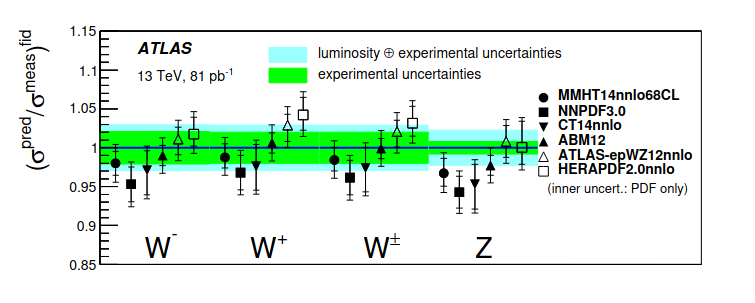
\includegraphics[scale=0.57]{chapter3/atlas13.png}\\
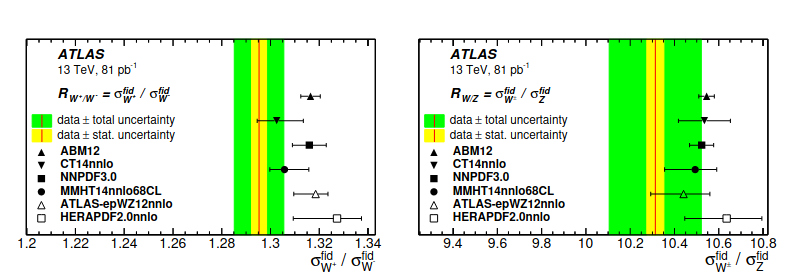
\includegraphics[scale=0.5]{chapter3/atlas13-1.png}
\end{tabular}
\caption{Ratio of Measured to predicted cross section(\textit{top}), comparison of measured and predicted cross section ratio of $W$ and $Z$ boson~(\textit{bottom}).~\cite{Aad_2016} }
\label{ratio-13tev}
\end{figure}


\begin{figure}[H]
\centering
\begin{tabular}{c}
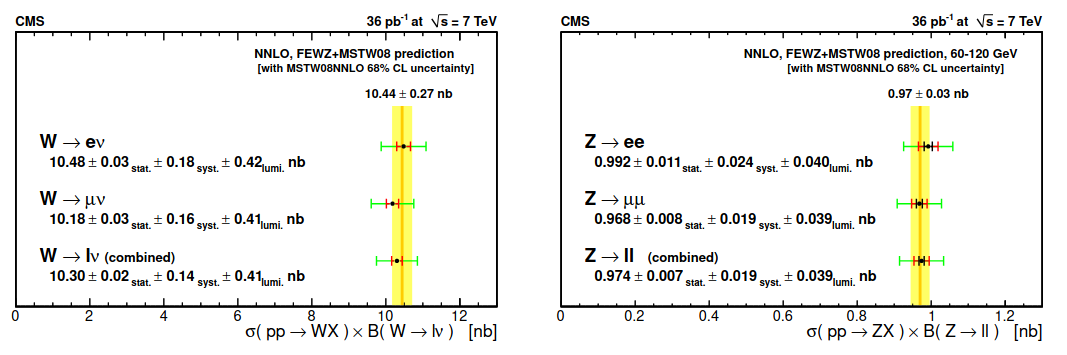
\includegraphics[scale=0.4]{chapter3/7tev1.png}\\
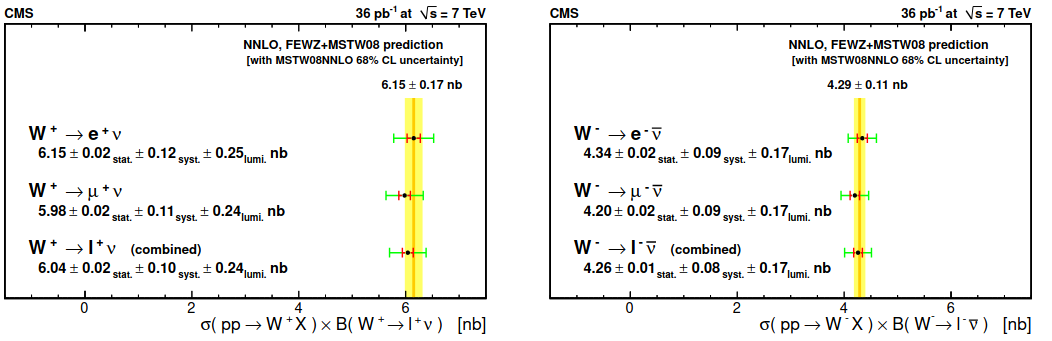
\includegraphics[scale=0.4]{chapter3/7tev2.png}\\
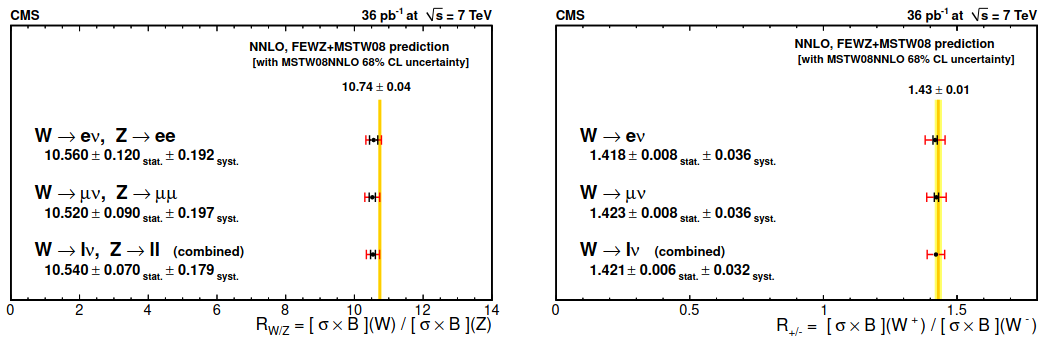
\includegraphics[scale=0.4]{chapter3/7tev3.png}
\end{tabular}
\caption{Measurements of vector boson cross section production multiplied with leptonic branching ratio~\textit{(top)}. Measurements of $W^{+}$ and $W^{-}$ production cross section times branching ratio~\textit{(middle)}. Ratio of $W^{+}$ to $Z$ and $W^{+}$ to $W^{-}$~\textit{bottom}. The yellow line showing the measured value with various experimental uncertainties at $7~TeV, 36~pb^{-1}$~\cite{2011}}
\label{7tev.data}
\end{figure}

Fig. \ref{ratio-13tev} shows the ratio of the experimentally measured and theoretically predicted cross section for the leptonic channel~($e$ and $\mu$) using various PDFs and also ratio of  production cross section of charged $W$ boson and $W^{\pm}$ boson to $Z$ boson compared to theoretical predictions with different PDF sets.

Fig.~\ref{7tev.data} shows the summary of the measurement in the electron and muon channels by CMS at $7~TeV$, and results are compared with the theoretical predictions. 


\begin{figure}[H]
\centering
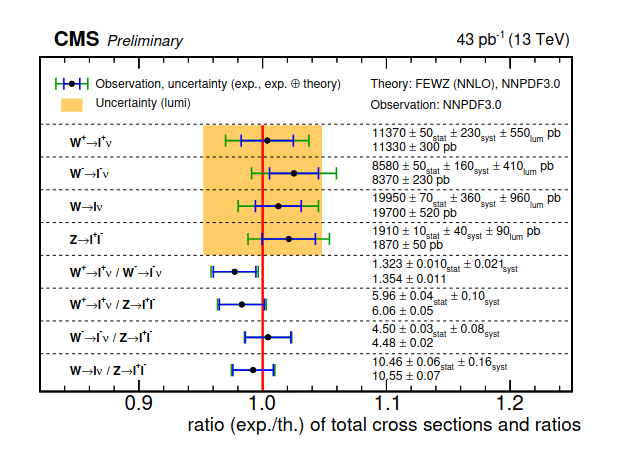
\includegraphics[scale=0.5]{chapter3/cms13.png}
\caption{The CMS measured total cross sections of $W$, $W^{+}$, $W^{-}$ and $Z$ boson times branching fraction and theoretically predicted cross section. In each column upper value represent measured cross section with uncertainties and lower value represent theoretically predicted cross section, and their ratio also.~\cite{CMS:2015ois}}       
\label{cms_comp}
\end{figure}
Figs.~\ref{cms_comp},~\ref{cms_comp1} and \ref{cms_comp2} shows the comparision of measurements at CMS with predictions by NNPDF3.0~(NNLO) at $13~TeV$.

\begin{figure}[H]
\centering
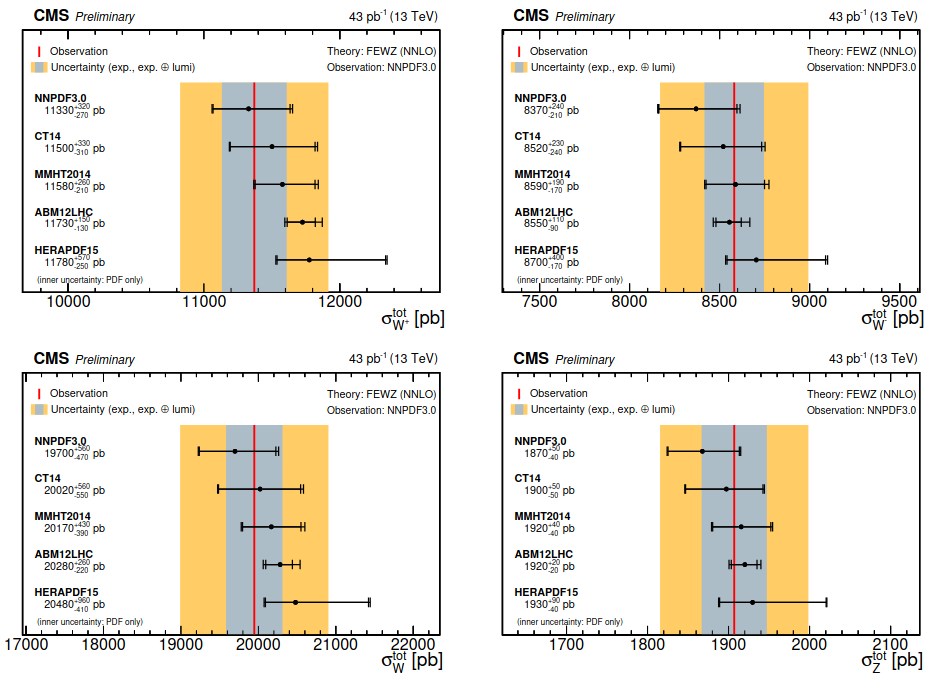
\includegraphics[scale=0.45]{chapter3/cms213.png}
\caption{Measured cross section ~(red line) and predicted cross section with different PDFs. The data points with error bars represent theoretically predicted value with various uncertainties~\cite{CMS:2015ois}}
\label{cms_comp1}
\end{figure}
\begin{figure}[H]
\centering
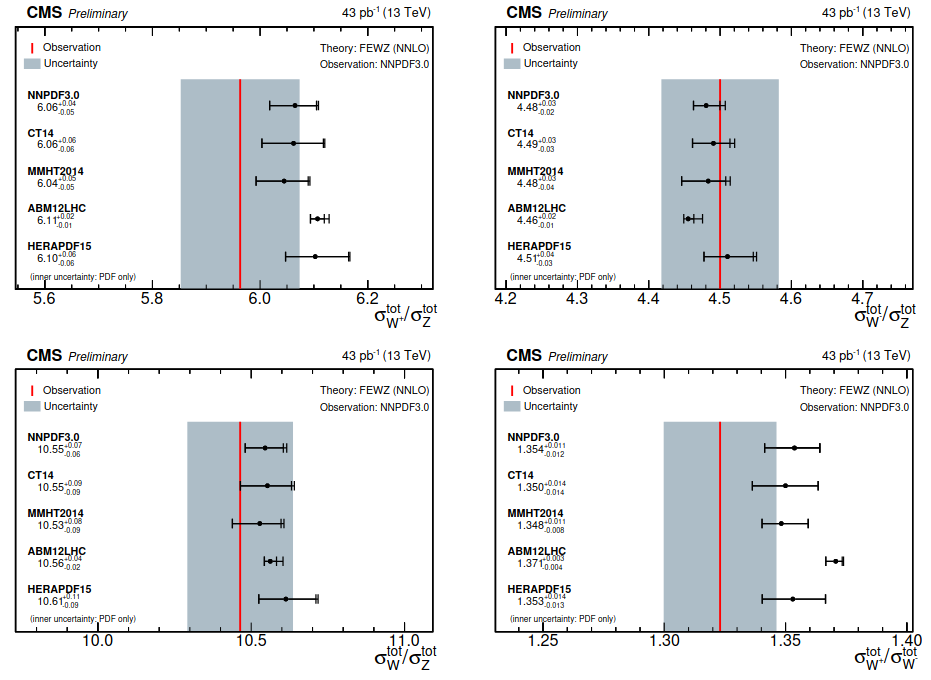
\includegraphics[scale=0.45]{chapter3/cms313.png}
\caption{Measured total  cross section ratios of vector bosons and predicted cross section ratios of vector boson with different PDFs set~\cite{CMS:2015ois}.}
\label{cms_comp2}
\end{figure}

\section{Uncertainties in the Predictions}
Imperfect knowledge of the proton parton distribution functions is the main source of uncertainties in predictions. The PDFs uncertainties can be evaluated from sum in quadrature by the difference of central PDF and Eigenvectors or error vectors of respective PDF set.\\
The uncertainties determination depends upon the given PDF set, for Monte Carlo set (NNPDF) uncertainties are determined differently from Hessian PDF  set and same for all other sets. 
\subsection{Computation of Hessian PDF uncertainties}
In hessian matrix approach the experimental uncertainties are propagated by diagonalising the $n\times n$ hessian matrix, more details can be found in~\cite{alekhin2011pdf4lhc}.

\textit{Hessian:} Consider a variable $Y$; the central value for $Y$ using central PDF is given by $Y_{0}$. $Y_{i}^{+}$ and $Y_{i}^{-}$ is the value of that variable corresponding to positive and negative direction of the error vector $i$ respectively~\cite{alekhin2011pdf4lhc}.  
\begin{eqnarray}
\Delta Y_{max}^{+}=\sqrt{\Sigma_{i=1}^{N}[max(Y_{i}^{+}-Y_{0},Y_{i}^{-}-Y_{0},0)]^{2}}\\
\Delta Y_{max}^{-}=\sqrt{\Sigma_{i=1}^{N}[max(Y_{0}-Y_{i}^{+},Y_{0}-Y_{i}^{-},0)]^{2}}
\end{eqnarray}
$\Delta Y^{+}$ is the PDF error which indicates increase in the observable $Y$, and $\Delta Y^{-}$ the PDF error indicates decrease in the observable $Y$. The sum is over all $N$ eigenvector directions.\\
\textit{Symmetric Hessian:} For the simple symmetric case where only the value of variable using central PDF $Y_{0}$ and $N$ error vector using PDF  $Y_{i}$, $(i = 1, . . . , N)$ are provided, the central value and PDF uncertainties are calculated as:
\begin{equation}
\Delta Y^{+}=\Delta Y^{-}=\Delta Y=\sqrt{\Sigma_{i=1}^{N}(Y_{i}-Y_{0})^{2}}
\end{equation}
\subsection{Computation of Monte Carlo PDF uncertainties}
For the NNPDF Monte Carlo set, a PDFs set with replicas is given. The average value for any observable $X$~(for example cross section) which depends on the PDFs sets is computed from usual formula:
\begin{equation}
<X(q)>~=~\frac{1}{N_{rep}}X_{i=1}^{N_{rep}}X(q^{i})
\end{equation}
where $N_{rep}$ is the number of replicas in the Monte Carlo PDF set. The associated uncertainty in the observable is found, according to the usual formula:
\begin{eqnarray}\label{sd}
\sigma_{X}~=~[\frac{N_{rep}}{N_{rep}-1}{\langle X(q)^{2}\rangle -\langle X(q)\rangle ^{2})}]^{1/2}\\
\sigma_{X}~=~[\frac{1}{N_{rep}-1}\Sigma_{i=1}^{N_{rep}}(X(q^{i})-\langle X(q) \rangle)^{2}]^{1/2}
\end{eqnarray}
NNPDF group provide both $N_{rep} = 100 $ and $N_{rep} = 1000$ replicas set. Equation \ref{sd} provides the 1–sigma PDF uncertainty on a general quantity which depends on PDFs.\\
Different PDFs groups provide both $68\%$ and $90\%$ confidence-level(C.L.) uncertainties. Some PDFs groups provide sets for both the $68\%$ confidence-level (C.L.) and $90\%$ C.L. Uncertainties. These uncertainties can be co-related by a factor of $1.64485$. In general we can evaluate PDFs uncertainties for both confidence level $68\%$ and $90\%$~i.e. NNPDF3.1~\cite{Watt_2011}.
\subsection{Theoretical Uncertainties}
The determination of theoretical uncertainties improves the PDFs relation to measurable quantities. The study of experimental uncertainties is much advanced than theoretical uncertainties, and only some of the theoretical uncertainties are explored in detail.\\
The determination ofstrong interactions between the quarks is the first source of theoretical uncertainty. The QCD parameters including the value of the strong coupling constant $\alpha_{s}$ and the heavy quark masses $m_{c}~(charm quarks)$ and $m_{b}~(bottom quark)$, and variation of re-normalisation $\mu_{R}$ and factorisation $\mu_{F}$ scales are the source of theoretical uncertainties.\\
Of these uncertainties, the uncertainty due to choice of strong coupling constant value $\alpha_{s}$ is explored in detail by each PDF group. The uncertainty due to choice of heavy quark masses~(charm and bottom) is also explored by some PDF groups~e.g. NNPDF3.1, Cteq18, HERA etc. The uncertainties due to variation in factorisation and re-normalisation scales are explored by NNPDF3.1.  
\subsubsection{The value of $\alpha_{s}$ ant its uncertainty}
The theoretical uncertainty due to the choice of strong coupling constant $\alpha_{s}$ value is studied and explored by each PDFs group. Different PDFs groups used different value of $\alpha_{s}$ as shown in Fig.~\ref{alpha}. The choice of $\alpha_{s}$ has clear importance for the PDFs prediction, especially for the gluons distribution.
\begin{figure}[H]
\centering
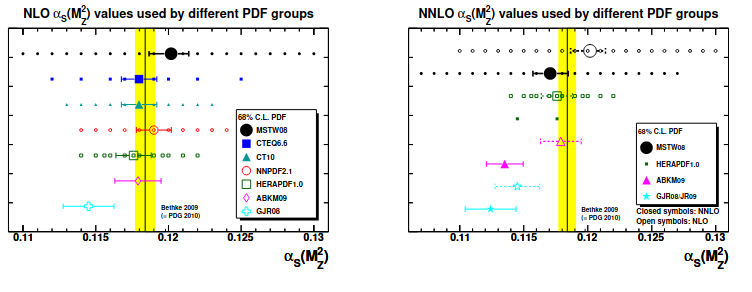
\includegraphics[scale=0.5]{chapter3/alpha.png}
\caption{The value of $\alpha_{s}$ used by different PDF groups}
\label{alpha}
\end{figure}
The values of $\alpha_{s}(m_{Z}^{2})$ and its uncertainties used by different PDFs  group are summarized in Fig.~\ref{alpha}. The world average value of $\alpha_{s}(m_{Z}^{2})$ is $\alpha_{s} = 0.1184 \pm 0.0007$~\cite{Martin_2009}.\\
The uncertainty on the value of $\alpha_{s}$, $\Delta\alpha_{s}=\pm0.001$ at $68\%$ C.L. and $\Delta\alpha_{s}=\pm0.002$ at $90\%$ C.L. has been used for the CTEQ, NNPDF studies. The predictions in the value of cross section changes with the choice of $\alpha_{s}$ value used. \\
\begin{figure}[h!]
\centering
\begin{tabular}{c}
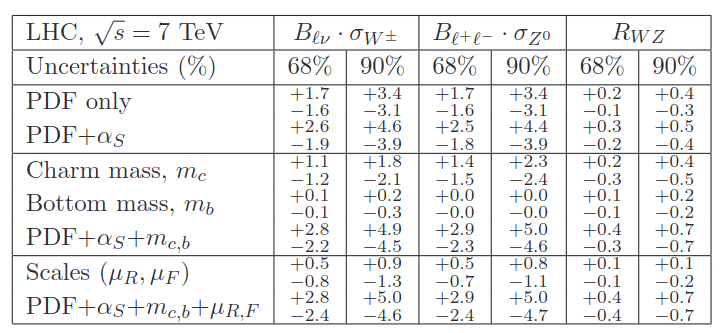
\includegraphics[scale=0.5]{chapter3/uncertain1.png}\\
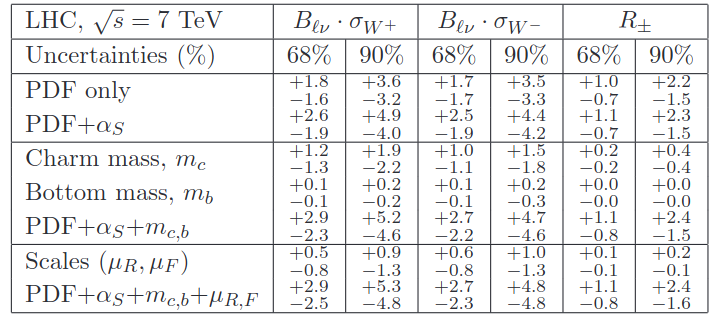
\includegraphics[scale=0.5]{chapter3/uncertain2.png}
\end{tabular}
\caption{Summary of theoretical uncertainties in prediction of $W$ and $Z$ boson cross-sections at 7TeV~\cite{Watt_2011}}
\vspace{2cm}
\label{uncertain}
\end{figure}
Various theoretical uncertainties for the $7~TeV$ are shown in Fig.~\ref{uncertain}.
\subsubsection{Computation of PDF+$\alpha_{s}$ uncertainties}
If PDF uncertainty and the $\alpha_{s}(m_{Z}^{2})$ uncertainty are correlated then PDF$+\alpha_{s}$ uncertainty at $68\%$~C.L. or 1-$\sigma$ uncertainty can be calculated. First calculate the 1-$\sigma$ PDF uncertainty at fixed $\alpha_{s}$ value, and then compute 1-$\sigma$ uncertainty in $\alpha_{s}$ with PDFs fixed at their central value, 1-$\sigma$ change in $\alpha_{s}$ corresponds to the change of 0.001 in its value and 2-$\sigma$ corresponds to the change of 0.002.\\
For example, if $\Delta\sigma_{PDF}$ is the PDF uncertainty in the cross section $\sigma$ and $\Delta_{\alpha_{s}(m_{Z}^{2})}\sigma$ is the $\alpha_{s}$ uncertainty, the combined PDFs$+\alpha_{s}$ uncertainty in $\Delta_{\sigma}$ is
\begin{equation}
\Delta\sigma~=~\sqrt{\Delta\sigma_{PDF}^{2}+\Delta\sigma_{\alpha_{s}}^{2}}
\end{equation}
Different PDFs groups used different strategies for computation of PDF+$\alpha_{s}$ uncertainty.
\subsubsection{NNPDF-Combined PDF and $\alpha_{s}$ uncertainties:}
For NNPDF3.1 PDFs, PDF set are given with value $\alpha_{s}$ in the range from 0.108 to 0.124 in step of $\Delta\alpha_{s}=0.002$ and few are also given with step of 0.001, for cross section which depends on the PDFs and the strong coupling  $\sigma(PDF, \alpha_{s})$, we have\\
\begin{equation}
(\delta\sigma)_{\alpha_{s}}^{\pm}~=~\sigma(PDF^{(\pm)},\alpha_{s}^{(0)}\pm\delta_{\alpha_{s}})-\sigma(PDF^{0},\alpha_{s}^{(0)})
\end{equation}\\
where PDF$^{\pm}$ is the value for the observable obtained when the value of  $\alpha_{s}$ is varied 0.001, i.e., $\alpha_{s}^{0}~\pm~\delta_{\alpha_{s}}$. The PDF+$\alpha_{s}$ uncertainty is\\
\begin{equation}
(\delta\sigma)_{PDF+\alpha_{s}}^{\pm}~=~\sqrt{[(\delta\sigma)_{\alpha_{s}}^{\pm}]^{2}+[(\delta\sigma)_{PDF}^{\pm}]^{2}}
\end{equation}
with $(\delta\sigma)_{PDF}^{\pm}$ is the PDF uncertainty on the observable $\sigma$ with the central value of $\alpha_{s}$. Figure~\ref{crossection7tev} shows the $W^{\pm}$ and $Z^{0}$ cross section, multiplied by the leptonic branching ratio and uncertainties in cross section predictions by different PDF groups.\\
The percentage uncertainties in the NNLO predictions at 7~TeV energy for both 68$\%$ and 90$\%$ confidence levels using MSTW08 PDFs is summarized in Fig.~\ref{uncertain}~for $W$, $W^{+}$, $W^{-}$, and $Z$ bosons production cross section. The uncertainty in cross section ratios are also predicted.

\begin{figure}[H]
\centering
\begin{tabular}{c}
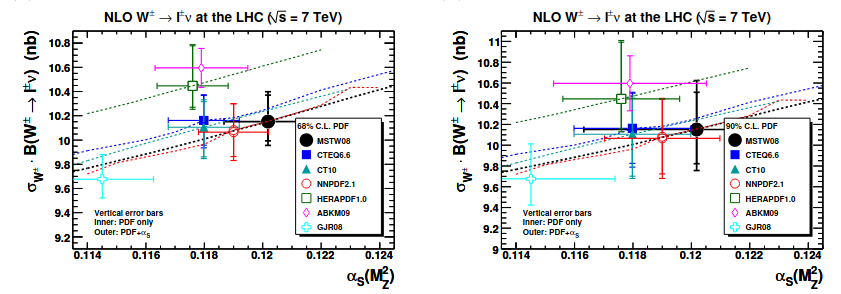
\includegraphics[scale=0.5]{chapter3/pdf-alpha.png}\\
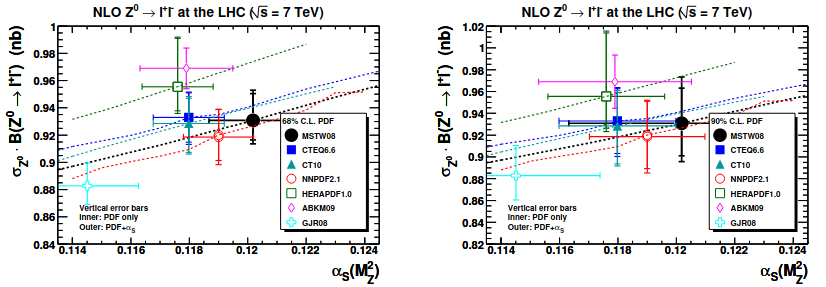
\includegraphics[scale=0.5]{chapter3/pdf-alpha1.png}
\end{tabular}
\caption{$W^{\pm}$ and $Z^{0}$ total cross sections, plotted as a function of $\alpha_{S}(M_{Z}^{2})$, at NLO.~\cite{Watt_2011}}
\label{crossection7tev}
\end{figure}








 

